%
% results_application.tex
%
One of the primary results of our architectural design is the BeeStream web application.  BeeStream was built using our architecture with the purpose of visualizing automated honeybee hive analytics data.  Figure \ref{fig:beestream-screenshot} shows Beestream's interface with data loaded.  We've made use of the architecture's modularity for data sources/channels, datapaths for data scaling, data filtering, data transmission protocols, charting component encapsulation, and dataset loading/missing data prevention.  BeeStream was built using the MEAN (MongoDB, Express, Angular, Node.js) web stack and illustrates how the architecture can leverage modern fullstack JavaScript's capabilities.  \par
\begin{figure}
  \centering
  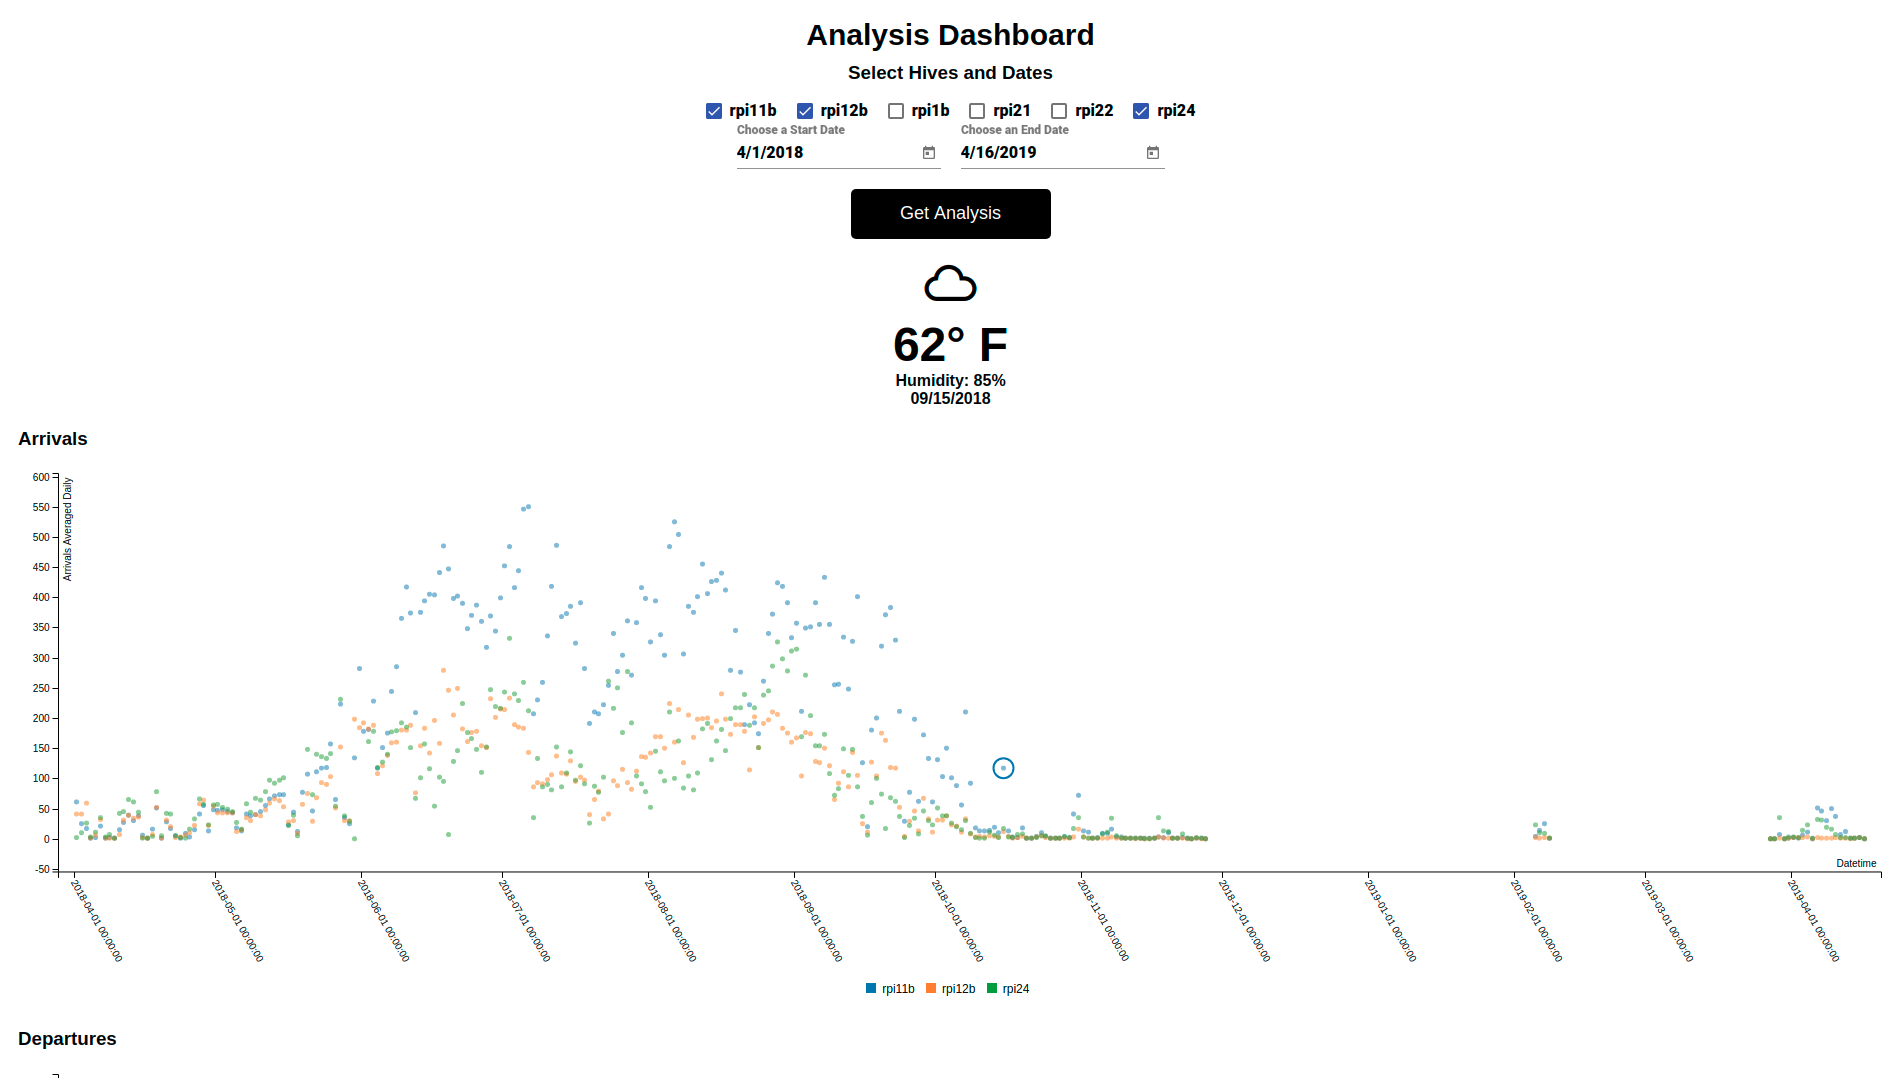
\includegraphics[width=6in]{images/beestream_screenshot.png}
  \caption{Beestream Screenshot}
  \label{fig:beestream-screenshot}
\end{figure}
Our archtectural implementation is also evident in the rendered web client.  The webpage is divided into a client driver and a series of rendered chart components as can be seen in Figure \ref{fig:beestream-screenshot-annotated}.  The client driver handles server-client communications, data filtering and requests, and the chart components' lifecycles as defined in our architecture.  Each of the chart components is dynamically rendered and populated only when data is present.  In our implementation, we chose to use C3.js \cite{c3js}, a package built on top of D3.js \cite{d3homepage} for our charting library.  As you can see in Figure \ref{fig:beestream-screenshot-annotated}, BeeStream includes a number of charts as well as a non-chart component, although the non-chart component is built to extent \textit{ChartComponent} so the driver doesn't know that this \textit{ChartComponent} doesn't define a chart.  This non-chart component is a weather widget shows the weather conditions for the point selected on the charts.  All charts use the driver to synchronize their currently selected point by having notifying the driver of a new selected point.  The driver distributes this notification to all \textit{ChartComponents}.
\begin{figure}
  \centering
  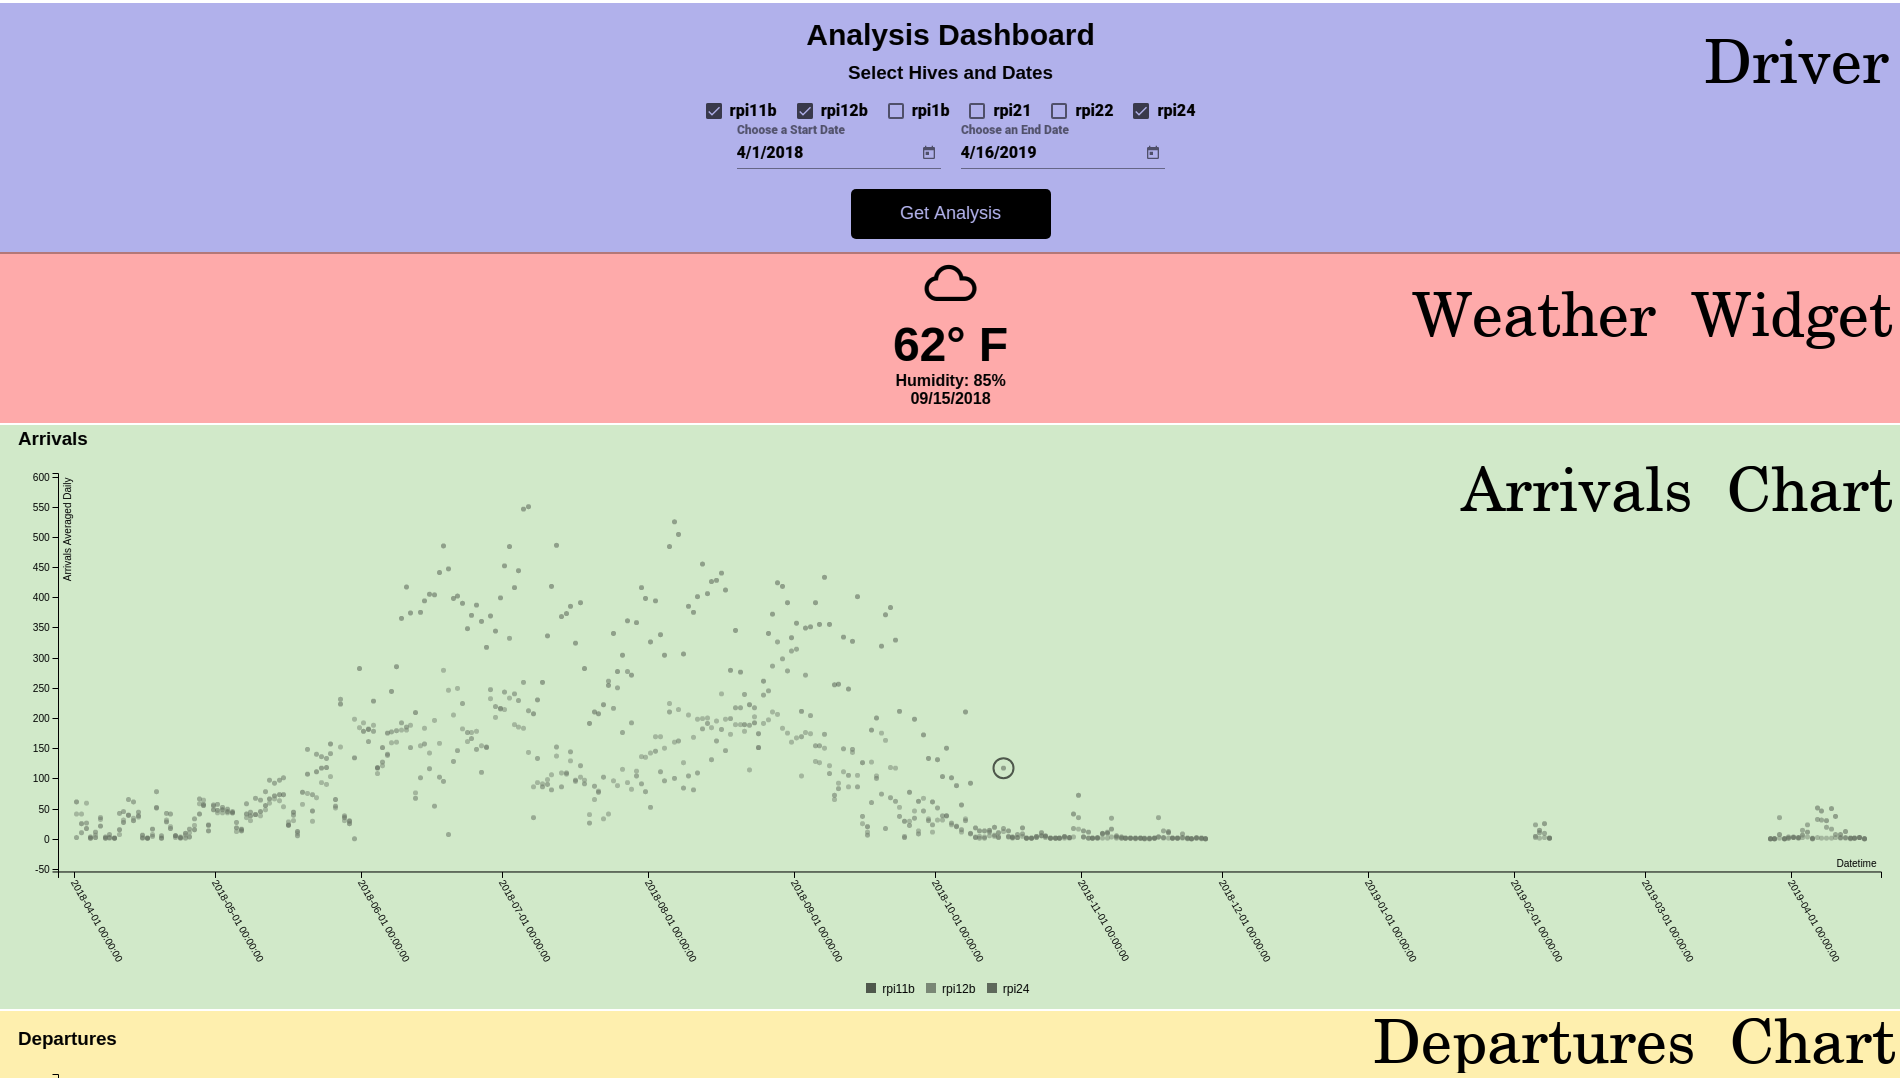
\includegraphics[width=6in]{images/beestream_screenshot_annotated.png}
  \caption{Beestream Screenshot with Annotations}
  \label{fig:beestream-screenshot-annotated}
\end{figure}
